\documentclass[ 12pt, xcolor=beamer,table,usenames,dvipsnames, ignorenonframetext, ngerman]{beamer}
\usetheme{Frankfurt}
\usecolortheme{dove}
\usepackage{appendixnumberbeamer}
%\setbeamersize{text margin left=20pt,text margin right=20pt,}
\useoutertheme{default}
\beamertemplatenavigationsymbolsempty 
\setbeamertemplate{headline}{}
\setbeamertemplate{itemize item}{\textbullet}

\addtobeamertemplate{navigation symbols}{}{
	\ifnum\insertframenumber>\inserttotalframenumber%
	\relax
	\else%
	\usebeamerfont{footline}%
	\usebeamercolor[fg]{footline}%
	\hspace{1em}%
	\insertframenumber
	\fi%
}
\setbeamercolor{footline}{fg=black}
\setbeamercolor{palette primary}{bg=blue!15,fg=black}
\setbeamercolor{background canvas}{bg=blue!5}
\setbeamercolor{palette secondary}{bg=blue!5}
\setbeamercolor{palette tertiary}{bg=blue!5}
\setbeamercolor{palette quaternary}{bg=blue!5}
\usepackage{soul}
\makeatletter
\let\HL\hl
\renewcommand\hl{%
	\let\set@color\beamerorig@set@color
	\let\reset@color\beamerorig@reset@color
	\HL}

\usepackage{tipa}
\usepackage{tikz}
\usetikzlibrary{shapes.geometric, arrows}
\mode<presentation>

\setbeamercovered{invisible}
\usepackage{multicol}
\usepackage[english]{babel}
\usepackage[latin1]{inputenc}
\usepackage{times}
\usepackage[T1]{fontenc}
\usepackage{ulem}
\usepackage{tipa}
\usepackage{qtree}
\usepackage{phonrule}
\usepackage{graphicx}
\usepackage{apacite}
\usepackage{xcolor}
\setlength\parindent{0pt}
\usepackage{natbib}
\usepackage{tikz}
\usetikzlibrary{arrows.meta}
\usepackage{tcolorbox}
\tcbuselibrary{raster}

\DeclareRobustCommand{\greencheck}{%
	\tikz\fill[scale=0.6, color=ForestGreen]
	(0,.35) -- (.25,0) -- (1,.7) -- (.25,.15) -- cycle;%
}
\title{Extending communication games to more players}
\author{Veronica Boyce}
\date{LangCog Lab Meeting}
\begin{document}

\begin{frame}
\maketitle
\pause
\begin{tikzpicture}[remember picture,overlay]
\node[xshift=1.5cm,yshift=1.2cm] at (current page.south west) {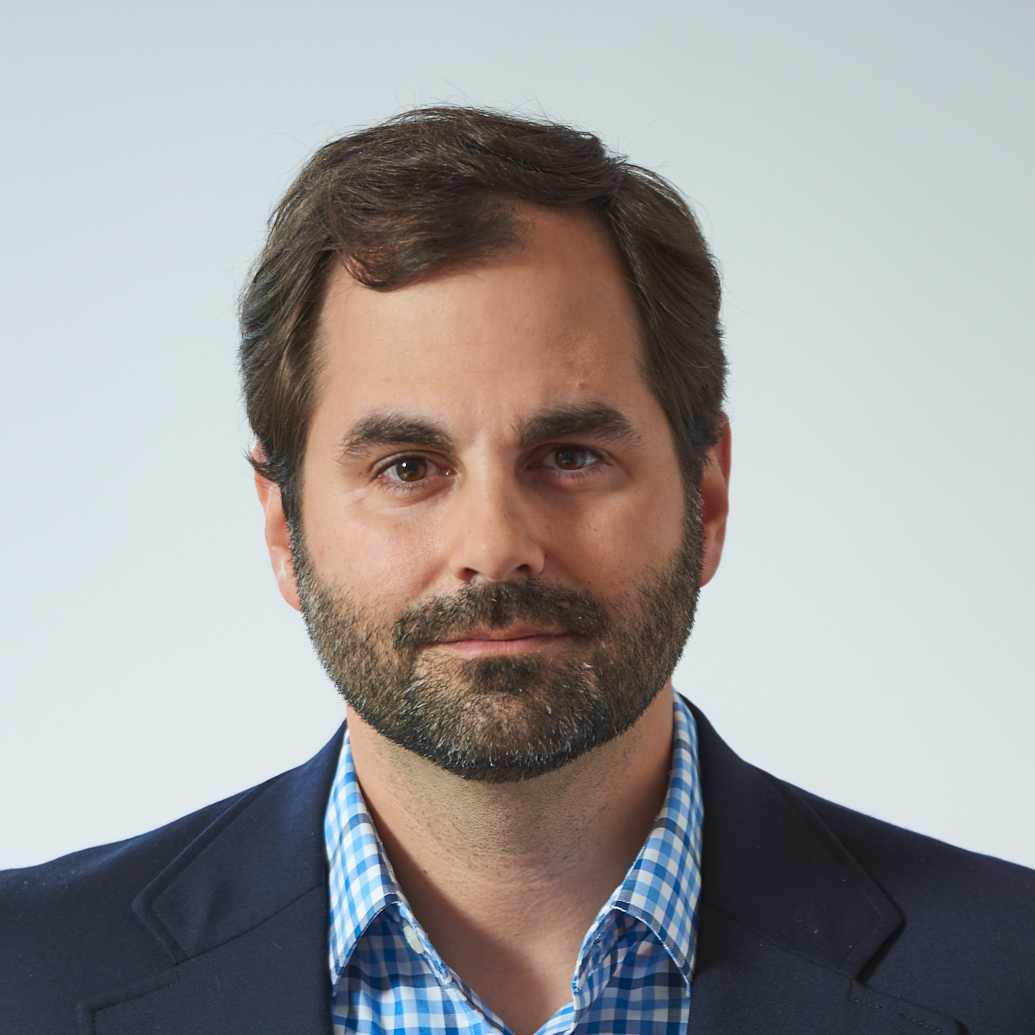
\includegraphics[width=.2\textwidth]{../images/mike.jpg}};
\node[xshift=-2.5cm,yshift=1.2cm] at (current page.south) {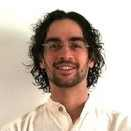
\includegraphics[width=.2\textwidth]{../images/noah.jpg}};
\node[xshift=0cm,yshift=1.2cm] at (current page.south) {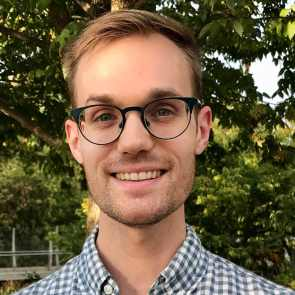
\includegraphics[width=.2\textwidth]{../images/robert.jpeg}};\pause
\node[xshift=-2.5cm,yshift=1.2cm] at (current page.south east) {
\includegraphics[width=.4\textwidth]{../images/hai.jpg}};
\end{tikzpicture}
\end{frame}

\begin{frame}
	BLAH BLAH  BIG PICTURE
\end{frame}

\begin{frame}{Clark \& Wilkes-Gibbs 1986}
	\pause
	\vspace{-.2cm}
	\begin{center}
		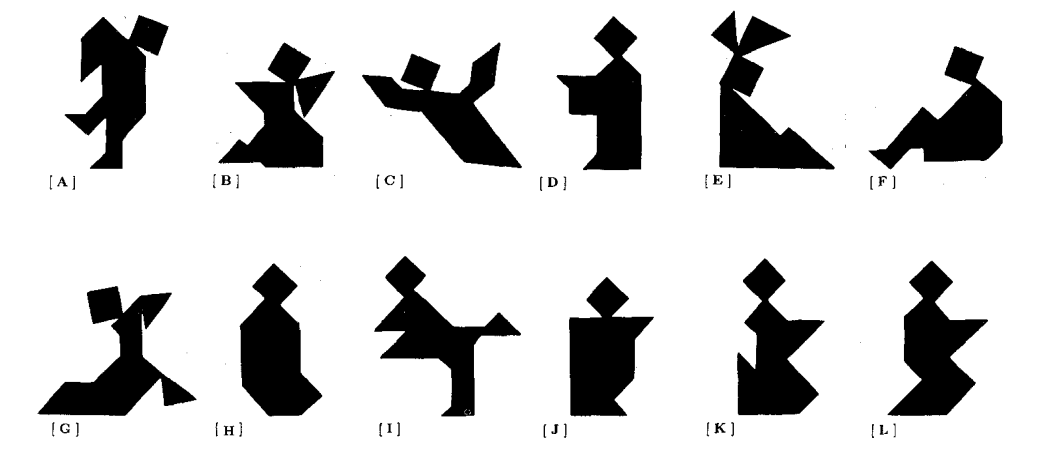
\includegraphics[width=.7\textwidth]{../images/clark_tangrams.png}
	\end{center}
	\vspace{-.4cm}
	\pause
	\begin{small}
		\begin{enumerate}
			\setlength{\itemsep}{-2pt}
			
			\item All right, the next one looks like a person who's ice skating, except, they're sticking two arms out in front. \pause
			\item Um, the next one's the person ice skating that has two arms? \pause
			\item The fourth one is the person ice skating, with two arms. \pause
			\item The next one's the ice skater. \pause
			\item The fourth one's the ice skater. \pause
			\item The ice skater.
		\end{enumerate}
	\end{small}
\end{frame}


\begin{frame}{Clark \& Wilkes-Gibbs 1986}
	
	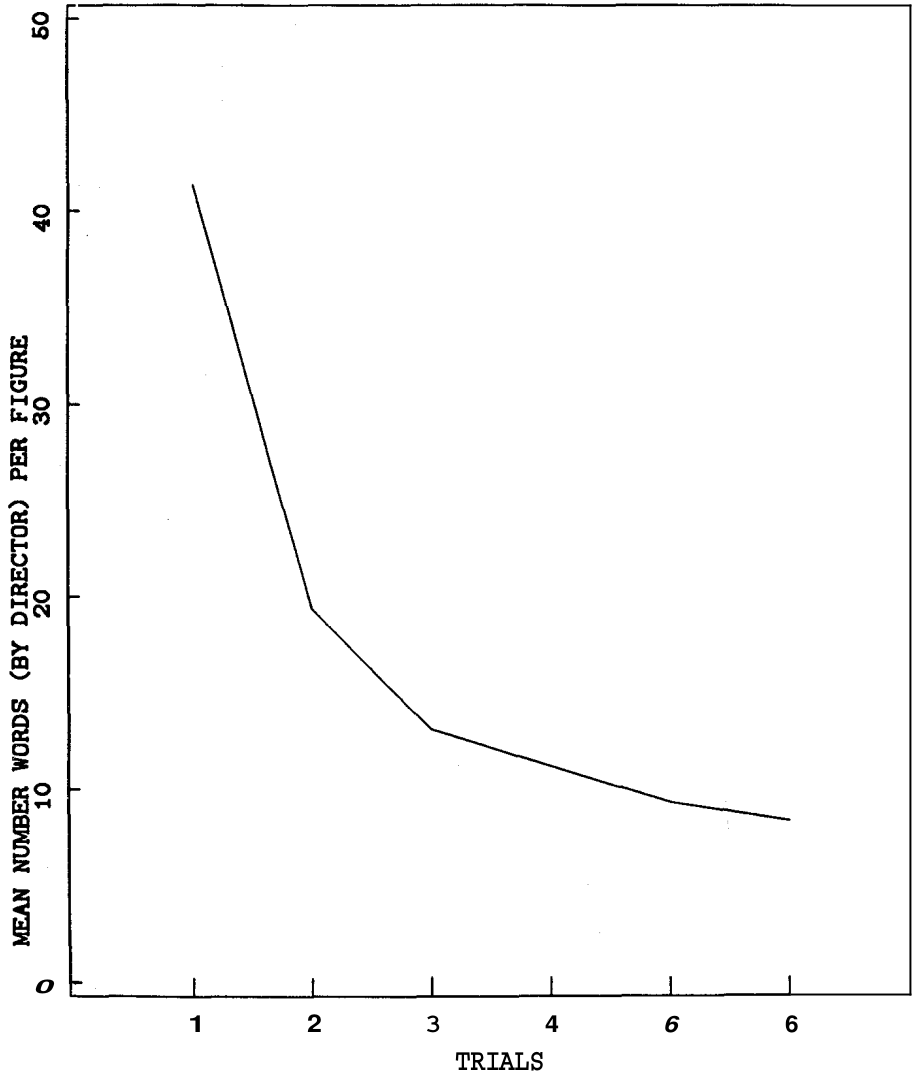
\includegraphics[width=.48\textwidth]{../images/clark_words.png}
	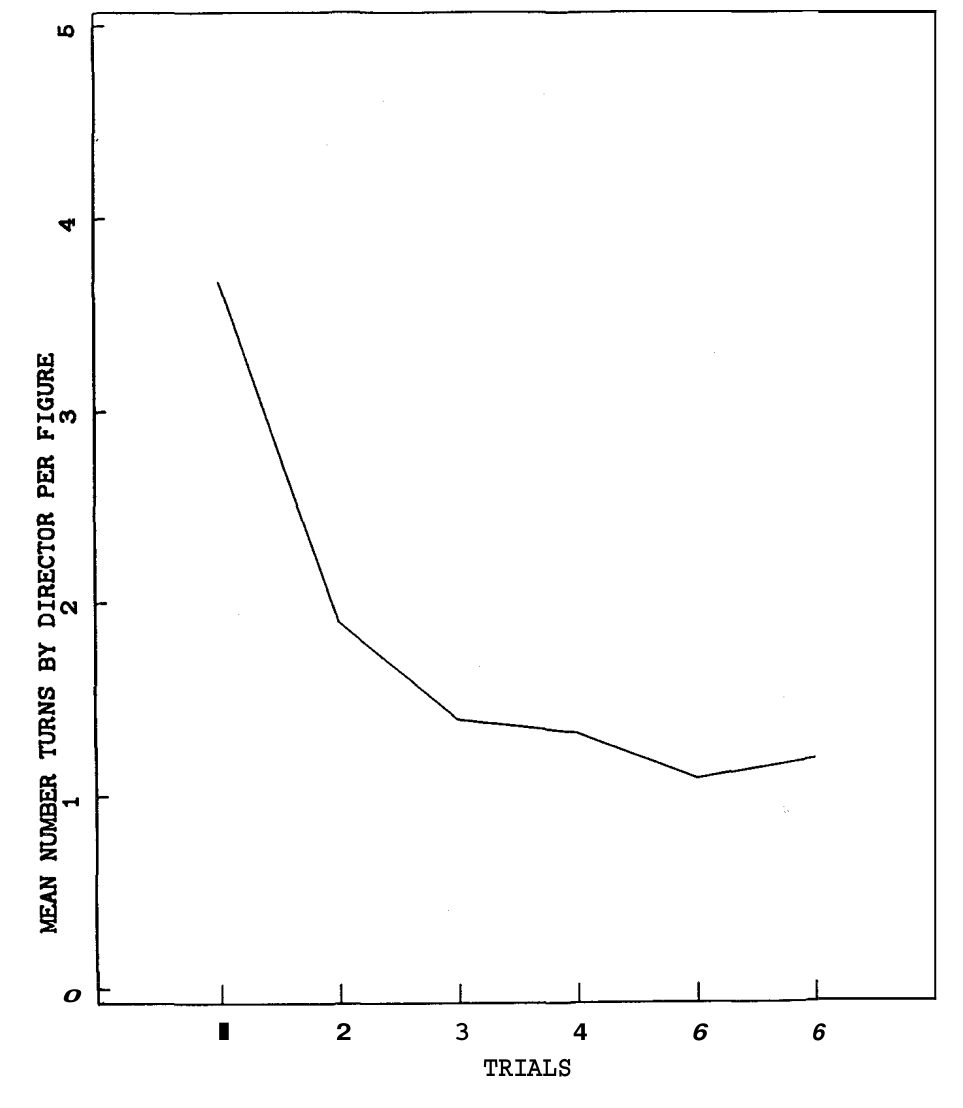
\includegraphics[width=.5\textwidth]{../images/clark_turns.png}	
	
\end{frame}

%\begin{frame}{Why study communication?}
%	BAD PART STARTS HERE
%
%	Verbal communication is a key method of human interaction.\\ 
%	% share ideas, teach each other, 
%	We communicate and understand more than surface meaning.\\ 
%	
%	Some of this is conventionalized, but some is dynamic. \\
%	
%%	Verbal communication is a key part of human interaction: we use it to ask for objects, teach
%%	facts to others, and express our feelings. We tailor our communication depending on who we are
%%	talking to according to our prior interactions with them, what words they know, and what they know
%%	about the topic being discussed. This adaptation is dynamic; over the course of a conversation,
%%	shared terminology and shorthands naturally arise.
%	
%\end{frame}

\begin{frame}{Partner-specific adaptation}\pause
		How do referring expressions develop?\pause
			\begin{itemize} 
		\item Mental modelling (ex. RSA) (Clark \& Wilkes-Gibbs 1986, Goodman \& Frank 2016) \pause
		\item Interactive Alignment Account -- bottom up priming (Garrod \& Pickering 2009)
	\end{itemize}\pause
	What are the speaker's strategies? \pause
	\begin{itemize}
		\item Audience design
		\item Common ground
		\item ``Aim Low'' (ex. Yoon \& Brown-Schmidt 2019)
	\end{itemize}

\end{frame}

%


%
\begin{frame}{Hawkins, Frank, \& Goodman 2020}
Scaling up with web-based experiments
\begin{itemize}
	\item Cued version with feedback on each trial \pause
	\item Message with a chat box \pause
	\item After all exclusions, 83 dyads \pause
\end{itemize}
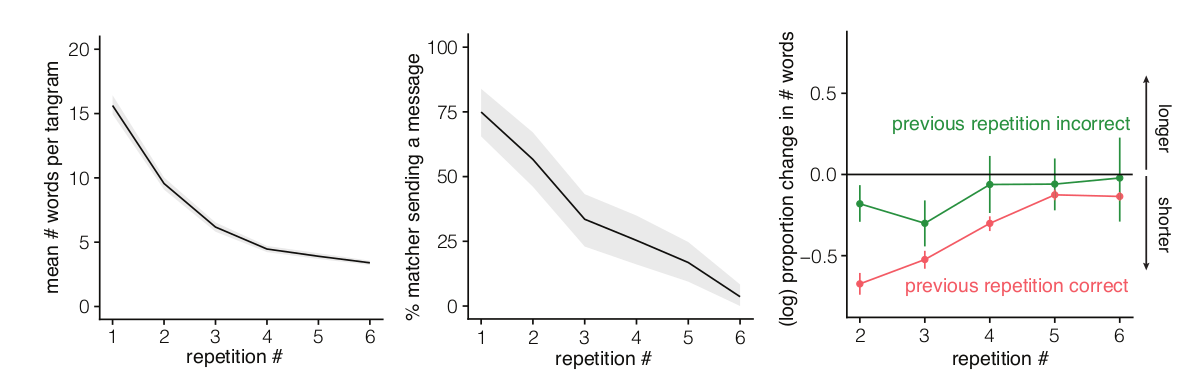
\includegraphics[width=\textwidth]{../images/hawkins_fewer_words.png}
\end{frame}
%


\begin{frame}{Hawkins, Frank, \& Goodman 2020}
	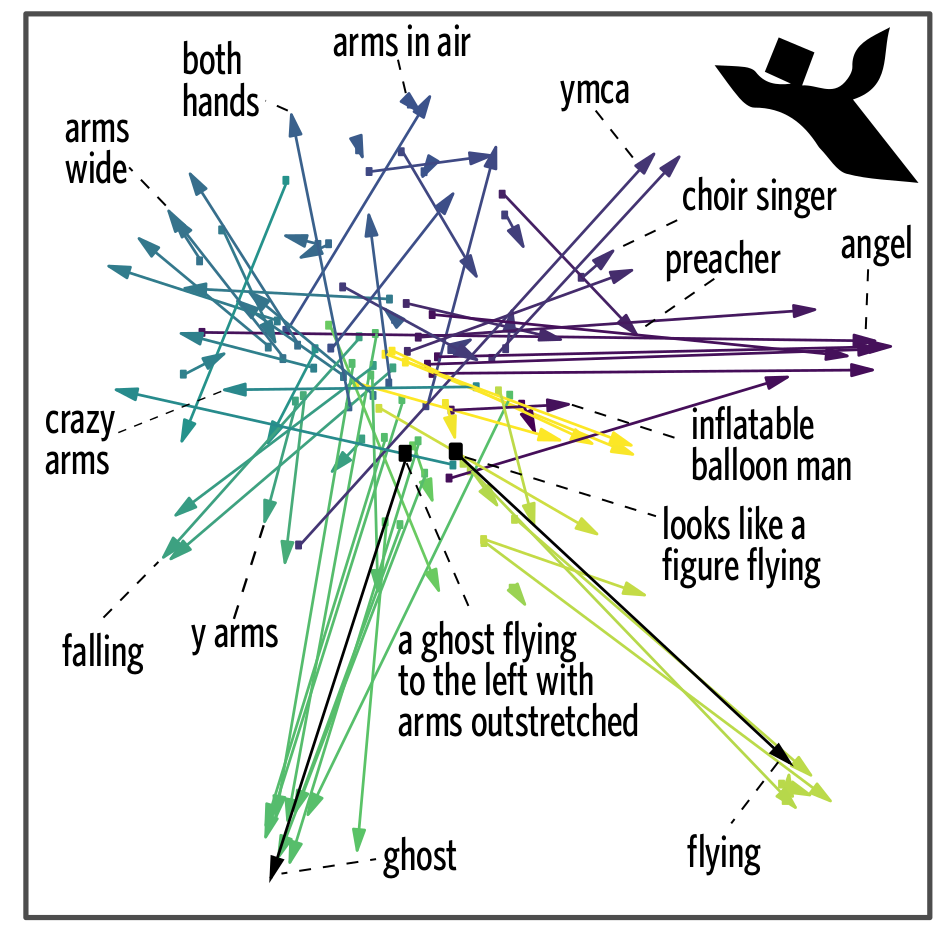
\includegraphics[width=.6\textwidth]{../images/hawkins_semantics.png}
	
	Semantics converge within and diverge between groups
\end{frame}

\begin{frame}{Weber \& Camerer 2003}
	\pause
	Two speaker/listener pairs train separately 
	
	Then `merger': speaker talks with *both* listeners \pause
	
	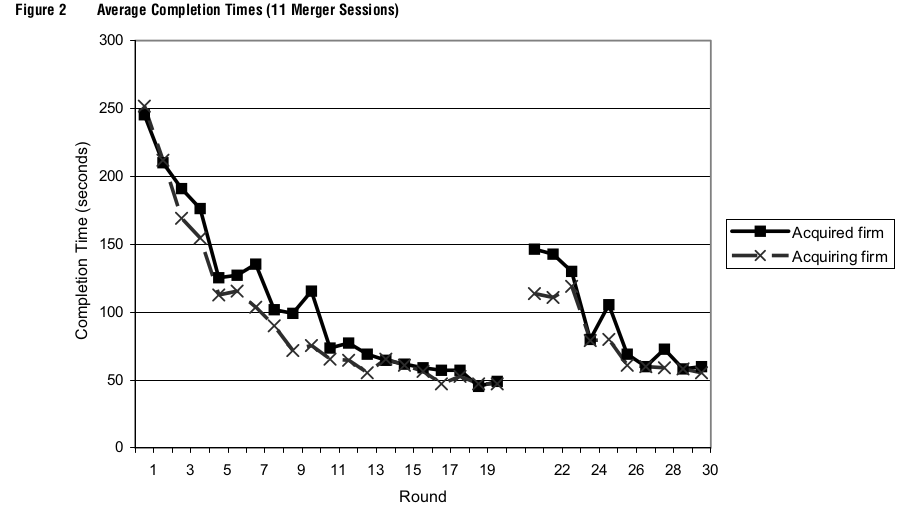
\includegraphics[width=\textwidth]{../images/weber.png}
	
\end{frame}

\begin{frame}{Yoon \& Brown-Schmidt 2019}
	Speaker talks to multiple matchers \\
	
	
	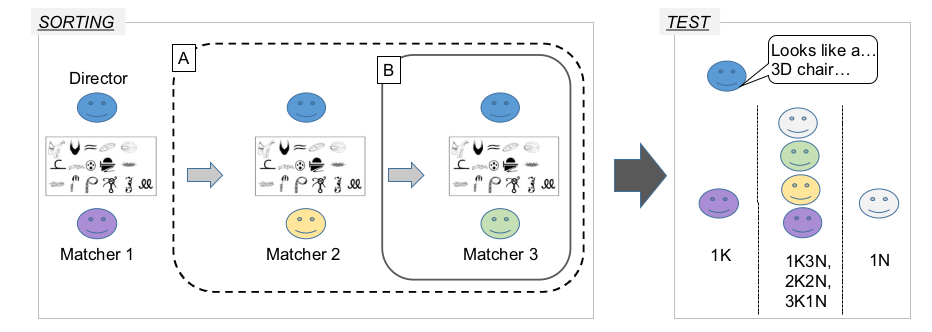
\includegraphics[width=\textwidth]{../images/yoon_diagram.png}
	
	Examine speaker's utterance length, elaborations, disfluencies
	%length, elaboration, disfluencies
\end{frame}

\begin{frame}
	END BAD PART
\end{frame}
%
\begin{frame}{First Year Project}
	Dynamics of alignment in larger groups \pause
	
	Compare groups of 2/3/4 communicators
	\begin{itemize}
		\item Look for differential reduction \pause
	\end{itemize} 
Rotate who is the knowledgeable speaker
\begin{itemize}
	\item Chosen for participant experience
	\item Stronger measure of alignment
\end{itemize}

\end{frame}

\begin{frame}{Experiment Framework}
Implemented in Empirica (Almaatouq et al 2020) 
%TODO describe what this is
 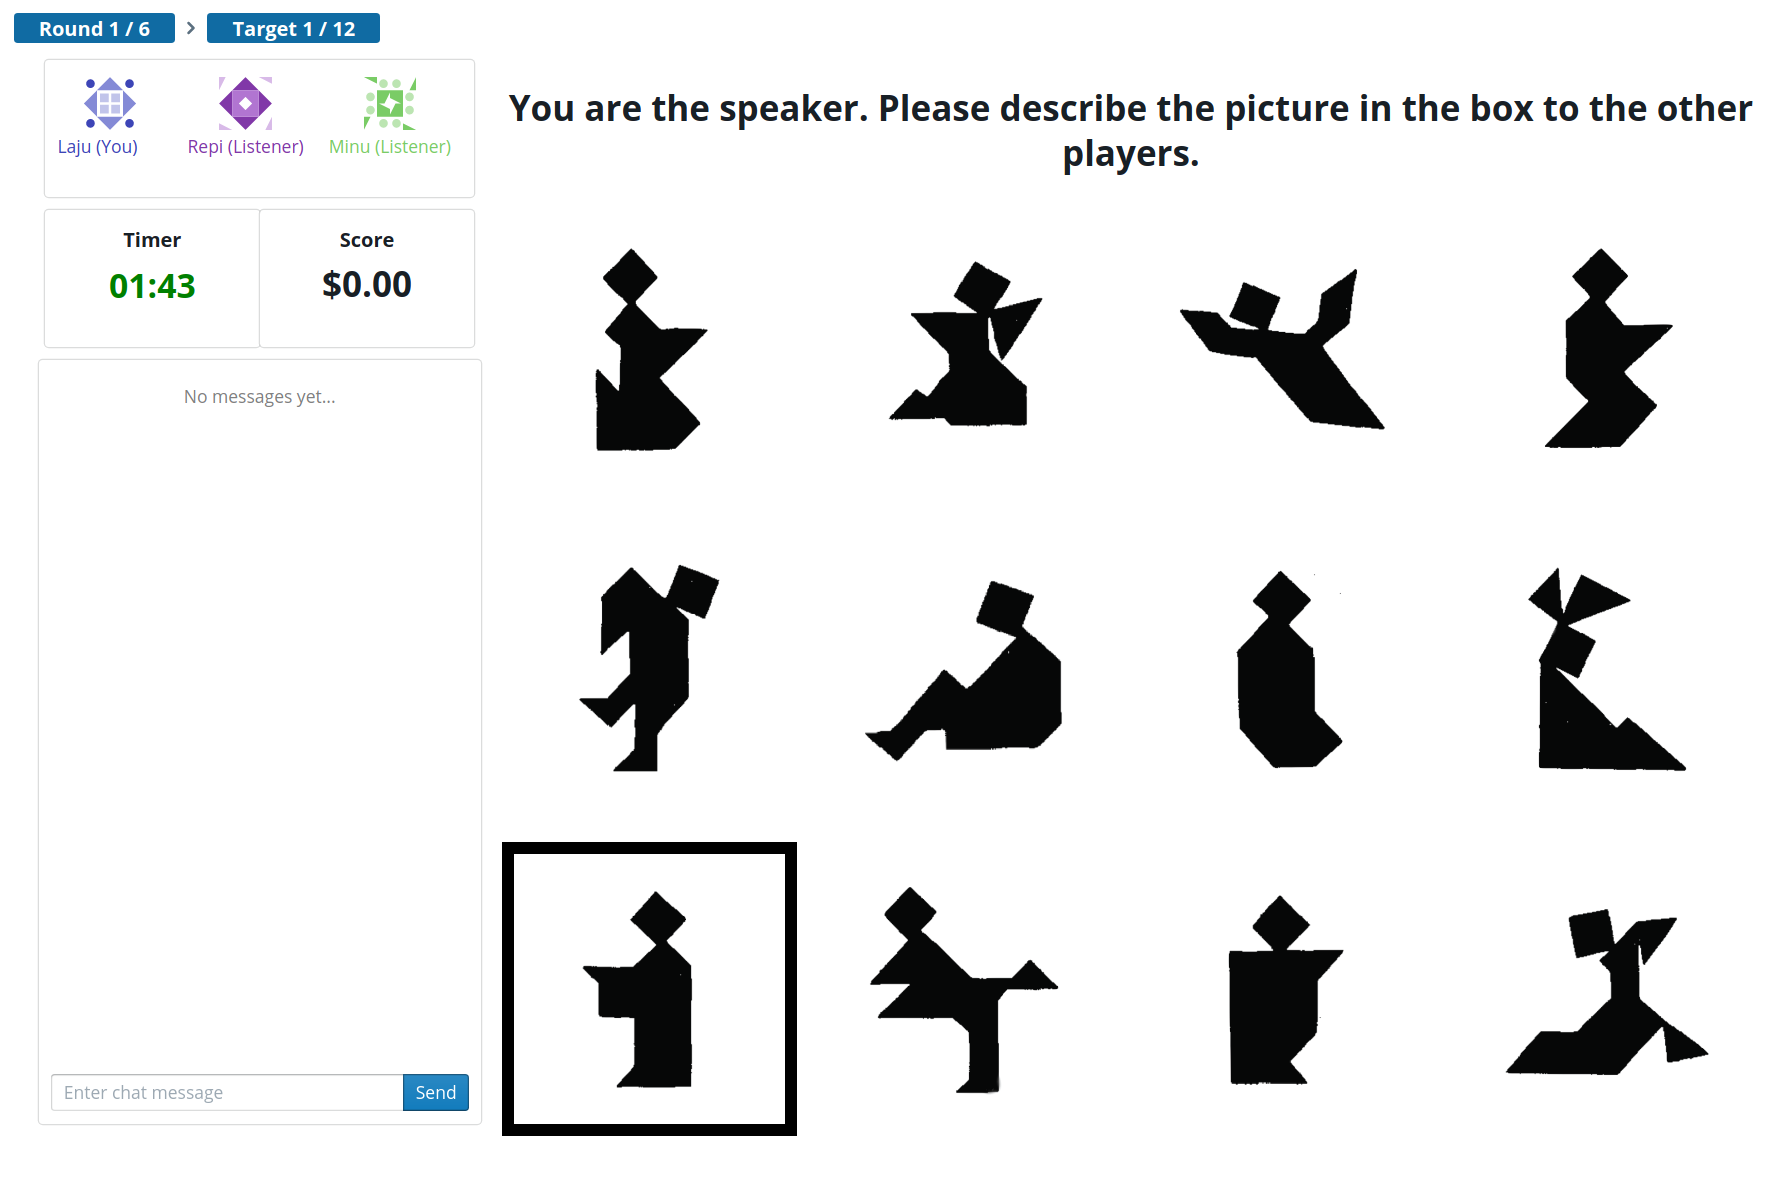
\includegraphics[width=\textwidth]{../images/interface.PNG}
\end{frame}

\begin{frame}{Experiment Framework}
	\only<1>{\begin{tikzpicture}[remember picture,overlay]
	\node[] at (current page.center) {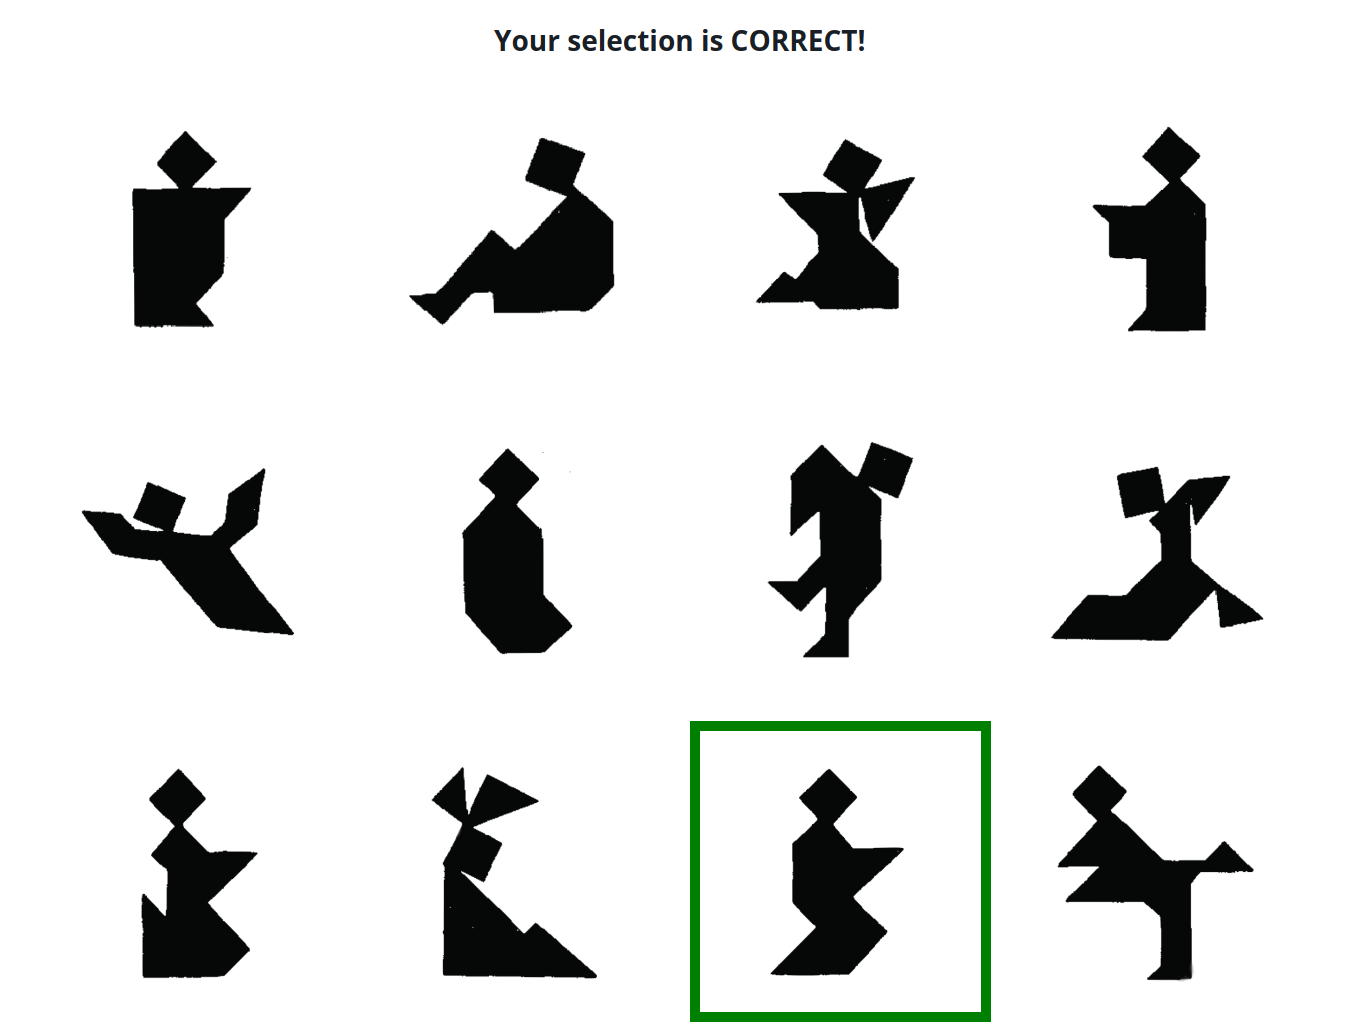
\includegraphics[width=.8\textwidth]{../images/listener_correct.png}};
		\node[yshift=1cm] at (current page.south) {Bonus: 4 points};
		\end{tikzpicture}}
\only<2>{\begin{tikzpicture}[remember picture,overlay]
\node[] at (current page.center) {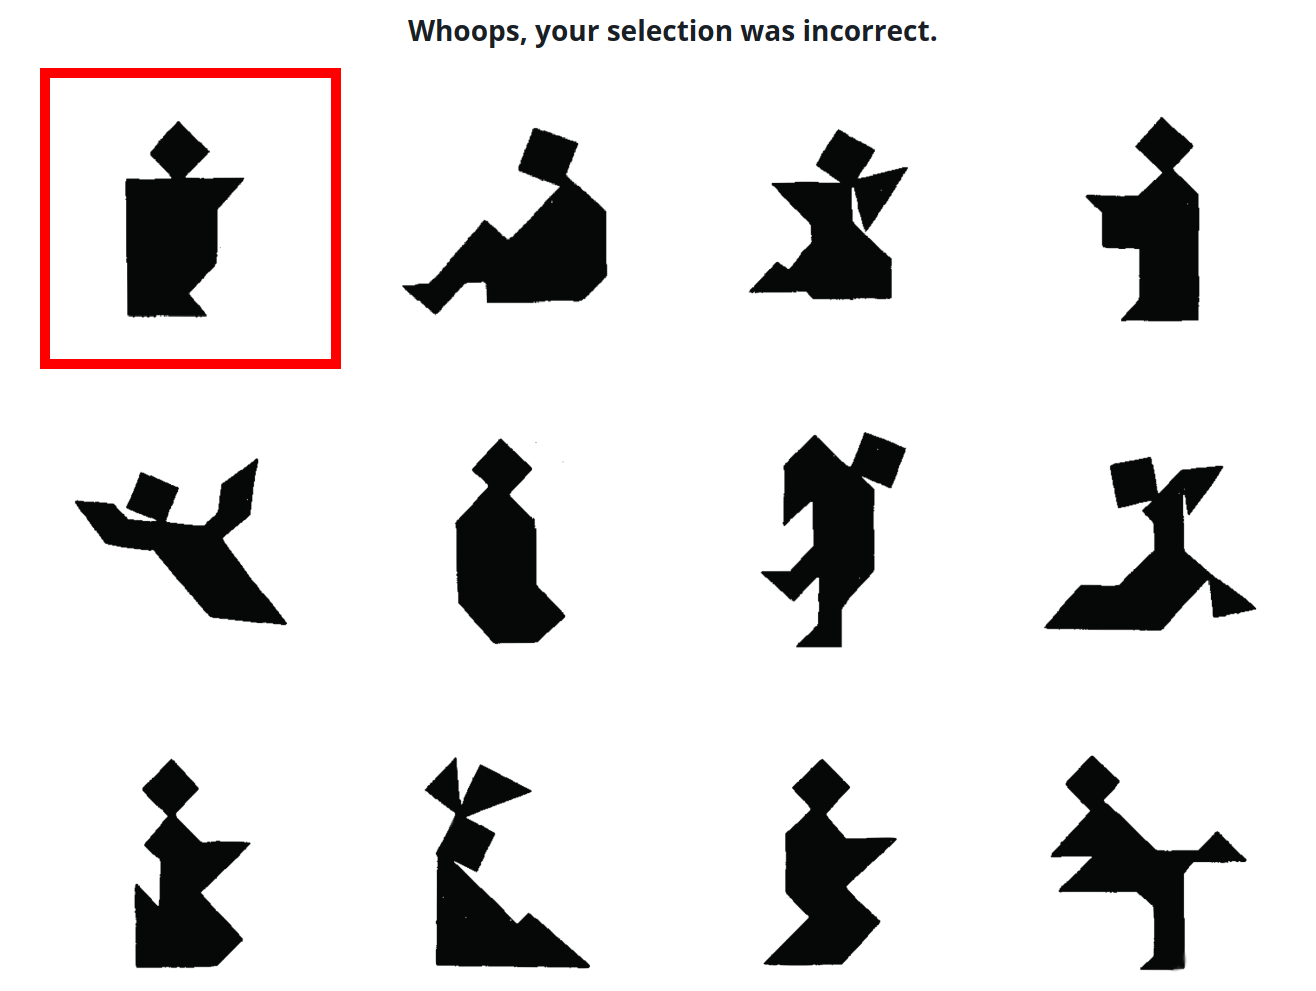
\includegraphics[width=.8\textwidth]{../images/listener_wrong.png}};
			\node[yshift=1cm] at (current page.south) {Bonus: 0 points};
			\end{tikzpicture}}
\only<3>{\begin{tikzpicture}[remember picture,overlay]
	\node[] at (current page.center) {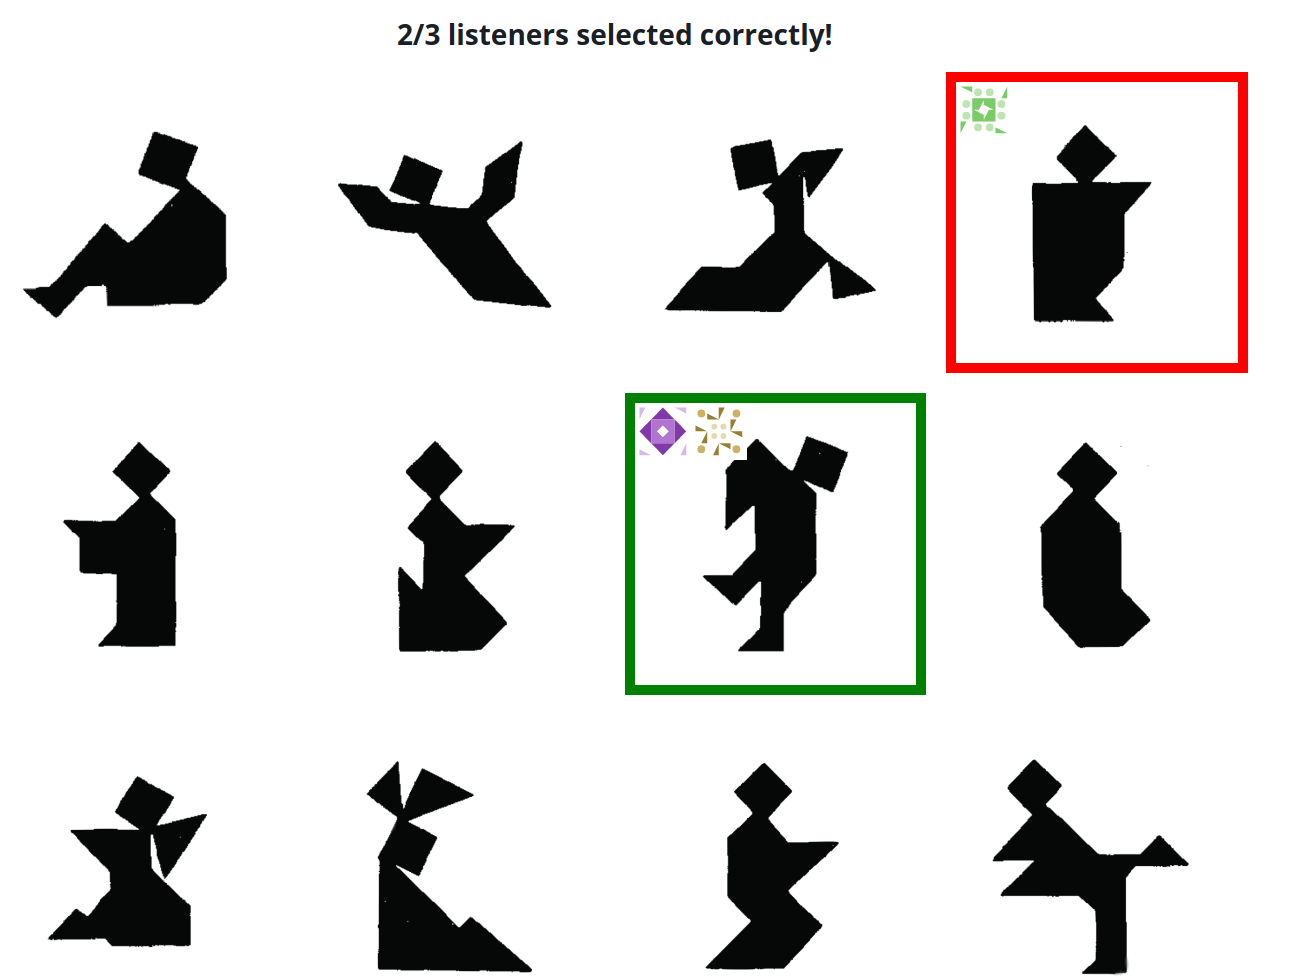
\includegraphics[width=.8\textwidth]{../images/speaker_feedback.png}};
\node[yshift=1cm] at (current page.south) {Bonus: Average of listeners = (2/3) * 4 points};

	\end{tikzpicture}}
\end{frame}
\begin{frame}{Recruitment}
	Goal: 20 games in each of 2/3/4-player conditions
	
	Each game has 6 blocks of 12 tangrams\pause
	
	\medskip
	
	Actual recruitment (over 3 days):
	\begin{itemize}
		\item 15 2-player games (+ 4 partial)
		\item 18 3-player games (+ 2 partial)
		\item 20 4-player games (+ 1 partial)
	\end{itemize}
Include all complete blocks

\end{frame}


\begin{frame}{Results:  Accuracy is high and increasing}
	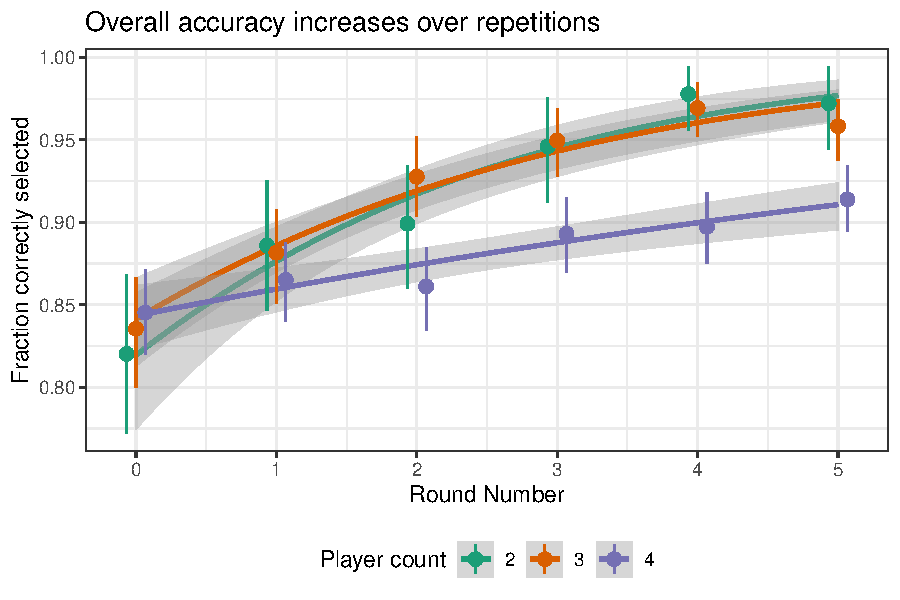
\includegraphics[width=\textwidth]{../images/accuracy.pdf}

\end{frame}

\begin{frame}{Results: 	Faster in later rounds}
	
	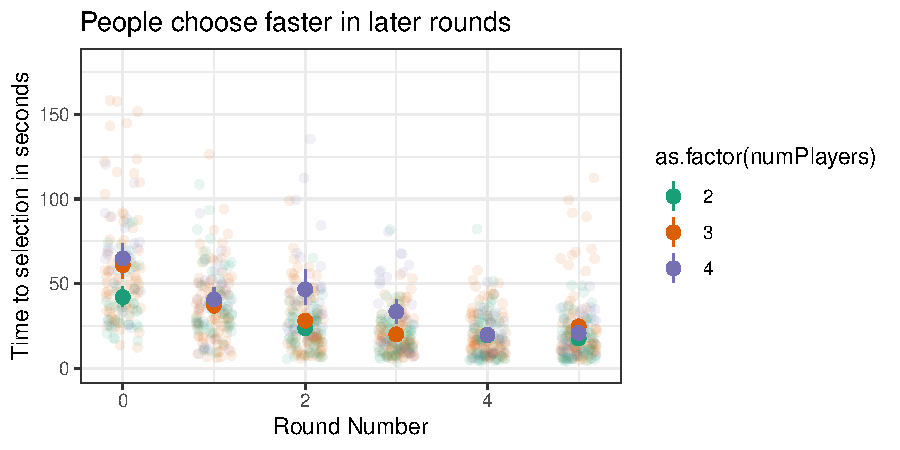
\includegraphics[width=\textwidth]{../images/time.pdf}


\end{frame}

\begin{frame}{Results: Reduction in words over time}
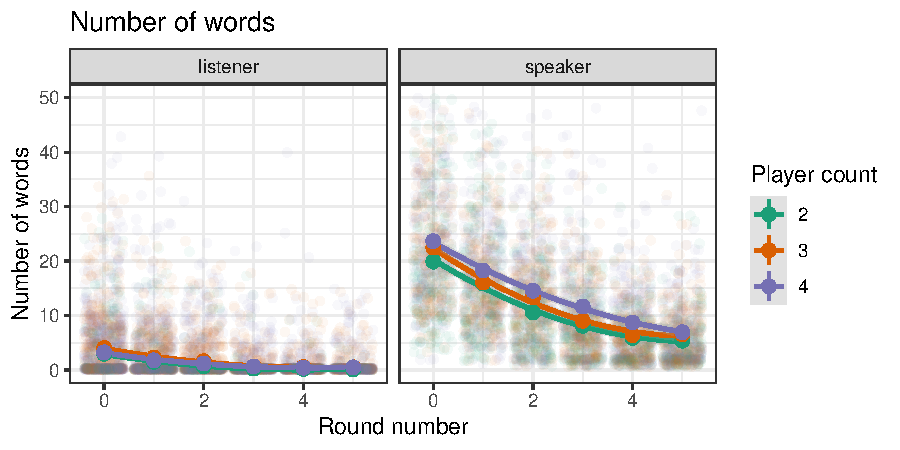
\includegraphics[width=\textwidth]{../images/words.pdf}


\end{frame}

\begin{frame}{Results: Variability in reduction rate}
	Most groups/tangrams reduce gradually
	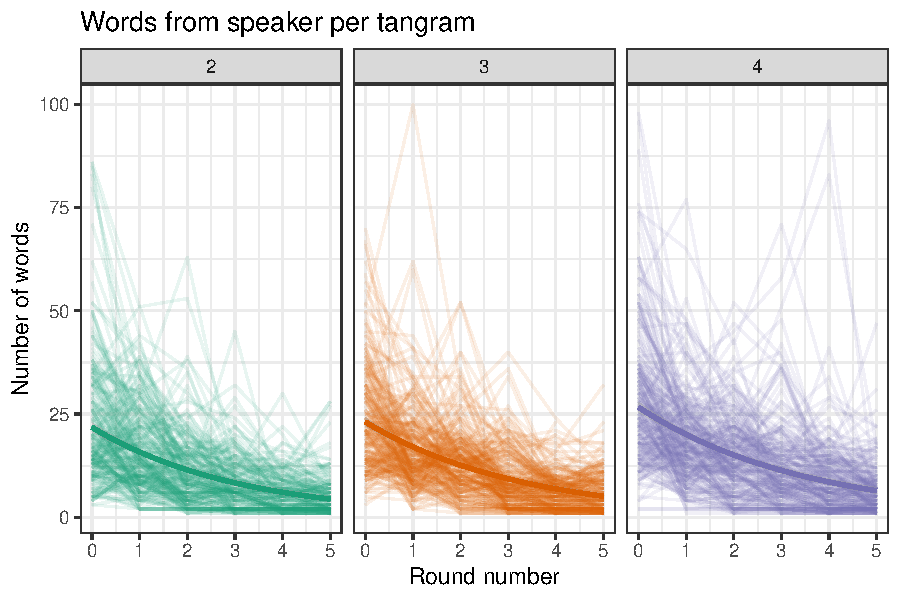
\includegraphics[width=\textwidth]{../images/words_lines.pdf}
\end{frame}

\begin{frame}{Results: Tangrams vary in nameability}
	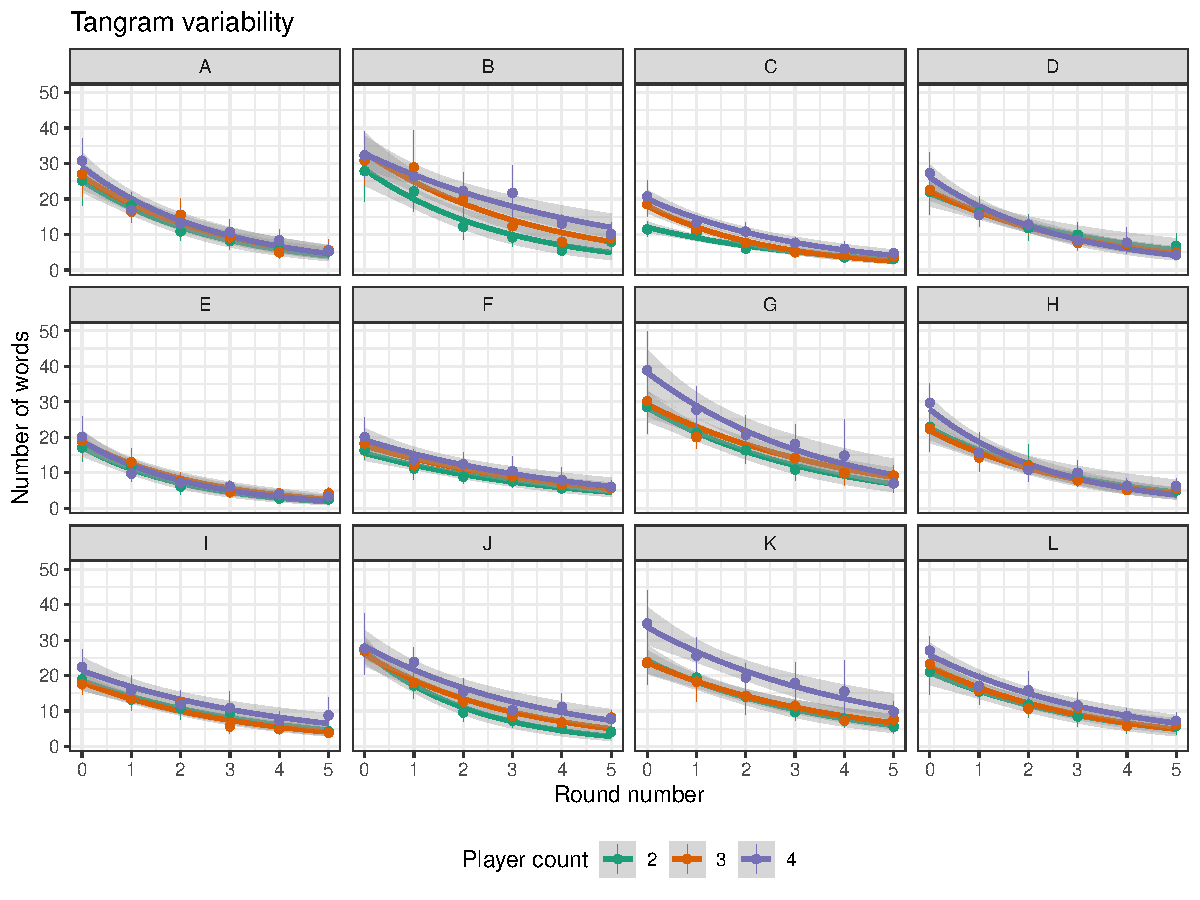
\includegraphics[width=\textwidth]{../images/words_tangrams.pdf}
\end{frame}

\begin{frame}{Example: iBaby}
	\begin{tikzpicture}[remember picture,overlay]
	\node[xshift=-1.5cm,yshift=-3cm] at (current page.north east) 
	{
\includegraphics[width=.2\textwidth]{../images/tangram_H.png}};
	\end{tikzpicture}
	
		\begin{enumerate}
			\setlength{\itemsep}{-2pt}
			\item A(S):Looks like a letter 'i'\\
			C: does it look like with its hand out or not\\
			B: \^{}\\
			A(S): no hand it is just a head and a body.\\
			C: oke\\
			A(S): more like a baby that has been swaddled in a blanket\\
			\item B(S): swaddled baby\\
			B(S): I\\
			B(S): i\\
			\item C(S): the baby i \\
			\item D(S): baby swaddled, looks like an i\\
			\item A(S): swaddled baby\\
			\item B(S): iBaby
		\end{enumerate}

\end{frame}


\begin{frame}{Example: Skydiving ghost superman}
	\begin{tikzpicture}[remember picture,overlay]
	\node[xshift=-1.5cm,yshift=-3cm] at (current page.north east) 
	{
\includegraphics[width=.2\textwidth]{../images/tangram_C.png}};
	\end{tikzpicture}
	\begin{enumerate}
		\setlength{\itemsep}{-2pt}
		\item A(S):flying man\\
		A(S): like superman \\
		A(S): hands in the air\\
		A(S): like skydiving
		\item B(S): the diver with no legs\\
		A: ok
		\item C(S): This one looks like a ghost to me, but you called it superman or skydiver\\
		A: ok no legs?\\
		C(S): Correct
		A: ok
		\item A(S): ghost, superman, skydiver
		\item B(S): sky diver, ghost\\
		A: ok\\
		\item C(S): Skydiving ghost superman
	\end{enumerate}
	
\end{frame}

\begin{frame}{Example: Karate kid}
	\begin{tikzpicture}[remember picture,overlay]
	\node[xshift=-1.5cm,yshift=-3cm] at (current page.north east) 
	{
\includegraphics[width=.2\textwidth]{../images/tangram_A.png}};
	\end{tikzpicture}
	\begin{enumerate}
		\setlength{\itemsep}{-2pt}
		\item A(S): Similar to the karate kid movie\\
		A(S): the crane kick\\
		B: Haha! Does it look like they have dangly sleeves!\\
		C: I don't know that one.\\
		A(S): yes\\
		D:yes i see, thats a good explenation.\\
	\end{enumerate}
	
\end{frame}

\begin{frame}{Example: Lack of shorthand}
	\begin{tikzpicture}[remember picture,overlay]
	\node[xshift=-.5cm,yshift=-2cm] at (current page.north east) 
	{
\includegraphics[width=.2\textwidth]{../images/tangram_J.png}};
	\end{tikzpicture}
	\vspace{-20pt}
	\begin{footnotesize}
	\begin{enumerate}
		\setlength{\itemsep}{-2pt}
		\item A(S):Diamond on top. Body with no real arms or legs. The body is shaped like a boot with the diamond on top.\\
		C: Is the boot pointed left or right?\\
		
		\item B(S): diamond on top, large body beneath it. Left is a straight line all the way down, small variations on the right to the main body\\
		\item C(S): Diamond in center on top. Left side straight, right side carved out like a vase.\\
		\item D(S): Diamond head, flat topped body, straight on the left side with two triangles pointing out on the left\\
		D(S): *on the right\\
		\item A(S): Diamond on top. Left side is straight, right side is obstructed, looks like a boot\\
		B: what do you mean by obstructed?\\
		A(S): The left side of the body is right, right side has bents in it	\\
		\item B(S): Diamond on top of a long large body/rectangle. Left side is complete, right side has bits missing
	\end{enumerate}
	\end{footnotesize}
\end{frame}



\begin{frame}{Example: Meta doesn't always help}
	\begin{tikzpicture}[remember picture,overlay]
	\node[xshift=-1cm,yshift=-2cm] at (current page.north east) 
	{
\includegraphics[width=.2\textwidth]{../images/tangram_L.png}};
	\end{tikzpicture}
	\vspace{-20pt}
	\begin{footnotesize}
		\begin{enumerate}
			\setlength{\itemsep}{-2pt}
			\item ...A(S): yes, the legs are like a zig zag\\
			C: CODE name ZIGZAG	\\
			A(S):	There are no legs upwards
			\item B(S): okay so similar to begger guy but no foot pointing up\\
			B(S): its like a zigzag\\
			B(S): i forgot the code name\\
			D: zigzag yea\\
			A: The one standing with knees bent	listener\\
			B(S): yeah\\
			B(S): standing \\
			C: Yeah zigzag
			\item C(S):	The begger with no foot coming out from the left\\
			B: zigzag\\
			C(S):	zigzag it is\\
			C(S):	sorry i forgot\\
			\item D(S):	zigzag
			\item A(S):	zigzag	
			\item B(S):	beggar guy\\
			B(S): zigzag
			
		\end{enumerate}
	\end{footnotesize}
\end{frame}
\begin{frame}{Future analyses: Semantics}
		\begin{tikzpicture}[remember picture,overlay]
	\node[xshift=-2.5cm,yshift=-3.2cm] at (current page.north east) 
		{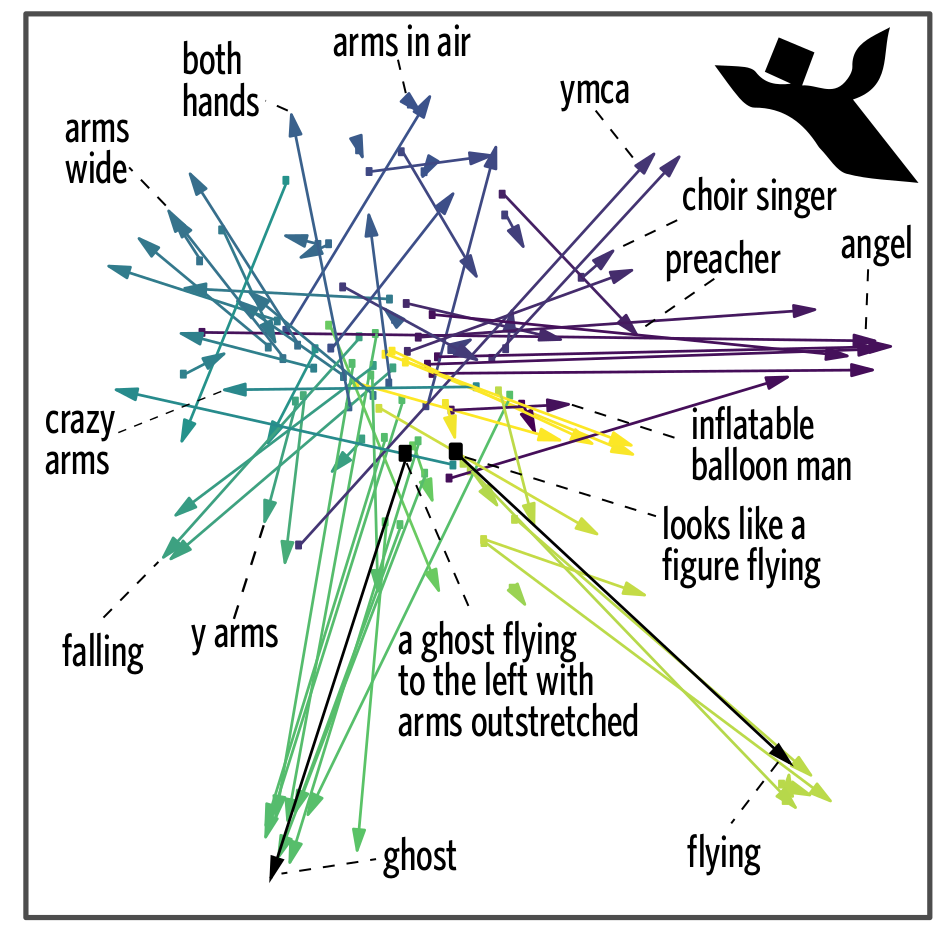
\includegraphics[width=.4\textwidth]{../images/hawkins_semantics.png}};
	\end{tikzpicture}

	\begin{itemize}
		\item Convergence by group size
		\item Accuracy \& convergence
		\item Geometric v metaphorical language
		\item Where/when are (atypical) concepts introduced?
	\end{itemize}
\end{frame}


\begin{frame}{Future directions}
How far does this generalize?
 \begin{itemize}
 	\item group size
 	\item item sets
 	\item game paradigms
 \end{itemize}
	
What makes communication more efficient?
\begin{itemize}
	\item Background knowledge
	\item Curriculum learning
\end{itemize}

\end{frame}

\begin{frame}{Comments, Questions?}
	Looking for feedback on
	\smallskip
	\begin{itemize}
	\item Analyses
	\item Future data sets
	\end{itemize}
\end{frame}

\appendix

%\begin{frame}{Hawkins, Frank, \& Goodman 2020}
%	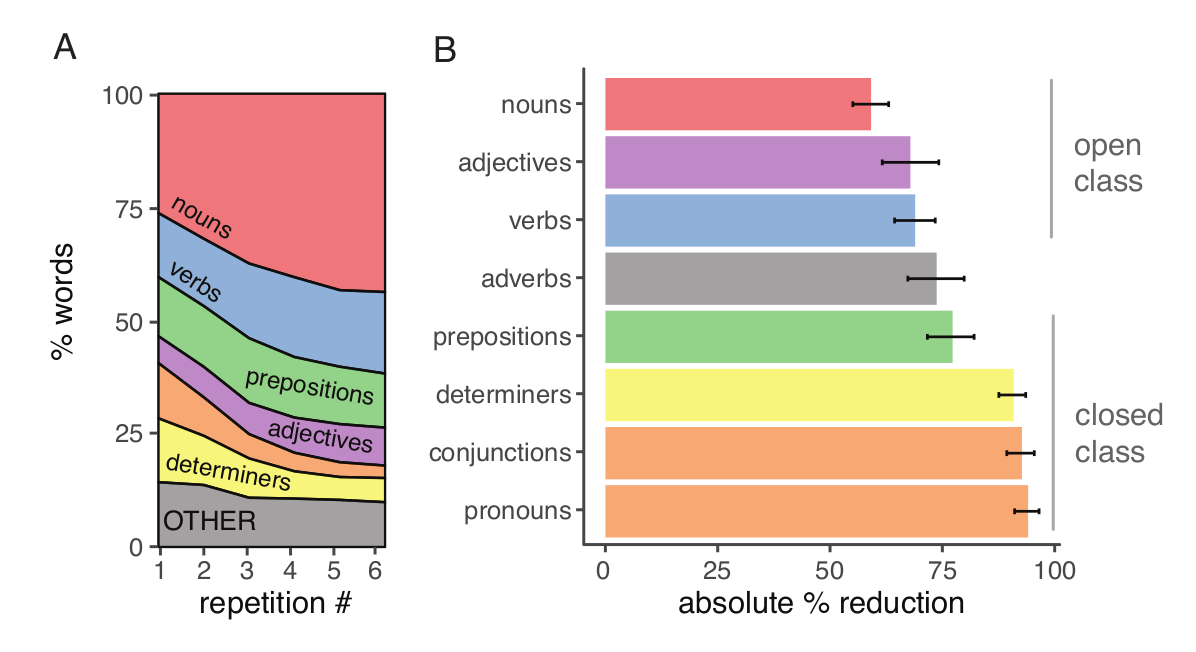
\includegraphics[width=\textwidth]{../images/hawkins_pos.png}
%	Words tend to drop out in syntactic units
%\end{frame}
\end{document}

